\documentclass[demonstration]{jfsma}

\usepackage[T1]{fontenc}
\usepackage{graphicx}
%\usepackage{color}
%\renewcommand\UrlFont{\color{blue}\rmfamily}
\usepackage{amsthm}
\usepackage{amsmath,amssymb,amsfonts}
\usepackage{tabularx}
\usepackage{caption}
\usepackage{listings}
% \usepackage{titlesec}
% \usepackage[english]{babel}
% \captionsetup{font=it}
\usepackage{ragged2e}
\usepackage{xurl}
\usepackage{hyperref}
\usepackage{pifont}
\usepackage{footmisc}
\usepackage{multirow}
\usepackage{enumitem}
\usepackage{algorithm2e}
\usepackage{float}
\usepackage{listings}
\usepackage{xcolor}
% \usepackage[inline, shortlabels]{enumitem}
% \usepackage[hyphens]{url}

\definecolor{codegreen}{rgb}{0,0.6,0}
\definecolor{codegray}{rgb}{0.5,0.5,0.5}
\definecolor{codepurple}{rgb}{0.58,0,0.82}
\definecolor{backcolour}{rgb}{0.95,0.95,0.92}
 
\lstdefinestyle{mystyle}{
    backgroundcolor=\color{backcolour},   
    commentstyle=\color{codegreen},
    keywordstyle=\color{magenta},
    numberstyle=\tiny\color{codegray},
    stringstyle=\color{codepurple},
    basicstyle=\footnotesize,
    breakatwhitespace=false,         
    breaklines=true,                 
    captionpos=b,                    
    keepspaces=true,                 
    numbers=left,                    
    numbersep=5pt,                  
    showspaces=false,                
    showstringspaces=false,
    showtabs=false,                  
    tabsize=2
}
 
\lstset{style=mystyle}

% --- Tickz
\usepackage{physics}
\usepackage{amsmath}
\usepackage{tikz}
\usepackage{mathdots}
\usepackage{yhmath}
\usepackage{cancel}
\usepackage{color}
\usepackage{siunitx}
\usepackage{array}
\usepackage{multirow}
\usepackage{amssymb}
\usepackage{gensymb}
\usepackage{tabularx}
\usepackage{extarrows}
\usepackage{booktabs}
\usetikzlibrary{fadings}
\usetikzlibrary{patterns}
\usetikzlibrary{shadows.blur}
\usetikzlibrary{shapes}

% ---------
% \usepackage{titlesec}
\usepackage{pdfpages}
\usepackage{booktabs}
\usepackage{csquotes}
\usepackage{lipsum}  
\usepackage{arydshln}
\usepackage{smartdiagram}
\usepackage[inkscapeformat=png]{svg}
\usepackage{textcomp}
\usepackage{tabularray}\UseTblrLibrary{varwidth}
\usepackage{xcolor}
\def\BibTeX{{\rm B\kern-.05em{\sc i\kern-.025em b}\kern-.08em
    T\kern-.1667em\lower.7ex\hbox{E}\kern-.125emX}}
\usepackage{cite}
\usepackage{amsmath}
\newcommand{\probP}{\text{I\kern-0.15em P}}
\usepackage{etoolbox}
\patchcmd{\thebibliography}{\section*{\refname}}{}{}{}

\setlength\tabcolsep{0.5pt}

\newcommand{\before}[1]{\textcolor{red}{#1}}
\newcommand{\after}[1]{\textcolor{green}{#1}}

\newcommand{\old}[1]{\textcolor{orange}{#1}}
\newcommand{\rem}[1]{\textcolor{red}{#1}}
\newcommand{\todo}[1]{\textcolor{orange}{\newline \textit{\textbf{TODO:} #1}} \newline \newline }



\newcounter{relation}
\setcounter{relation}{0}
\renewcommand{\therelation}{\arabic{relation}}
\newcommand{\relationautorefname}{Relation}

\newenvironment{relation}[1][]{%
    \refstepcounter{relation}%
    \noindent \raggedright \textit{\textbf{Relation. \therelation}} \hfill$}
{%
$ \hfill \phantom{x}

}

\newcounter{proof}
\setcounter{proof}{0}
\renewcommand{\theproof}{\arabic{proof}}
\newcommand{\proofautorefname}{Proof}

\renewenvironment{proof}[1][]{
    \refstepcounter{proof}
    \noindent \raggedright \textit{\textbf{Proof. \theproof}}

    \setlength{\leftskip}{1em}

}
{

\
\setlength{\leftskip}{0pt}
}


\titre{Une Aide à la Conception de SMA par Apprentissage par Renforcement et Modélisation Organisationnelle}


\auteur{Julien Soulé\up{a,b}}{julien.soule@lcis.grenoble-inp.fr}
\auteur{Jean-Paul Jamont\up{a}}{jean-paul.jamont@lcis.grenoble-inp.fr}
\auteur{Michel Occello\up{a}}{michel.occello@lcis.grenoble-inp.fr}
%%%Si besoin d'ajouter des auteurs à la ligne :
\auteurSuite{Louis-Marie Traonouez\up{b}}{louis-marie.traonouez@thalesgroup.com}
\auteurSuite{Paul Théron\up{c}}{paul.theron@orange.fr}

\institution{\up{a}%
  Univ. Grenoble Alpes, Grenoble INP, LCIS, 26000, Valence, France}
\institution{\up{b}%
  Thales Land and Air Systems, BU IAS, Rennes, France}
\institution{\up{c}%
  AICA IWG, La Guillermie, Franc}

% TODO: est-ce qu'on peut utiliser "dissemination" alors que le papier AIAI n'est pas publié à proprement parler?

\begin{document}

\maketitle

\begin{resume}

  % Contexte
  La conception d'un SMA peut être vue au travers de son organisation englobant les interactions individuelles jusqu'aux stratégies collectives.
  %Il s'agit alors de chercher une organisation permettant d'atteindre l'objectif donné de façon optimale sous des contraintes organisationelles données ou de l'environnement.
  % Problème
  Une approche empirique de recherche d'une organisation adéquate sur certains environments peut s'averer coûteuse en raison de leur manque d'appréhension ou leur complexité.
  % Contribution
  PRAHOM augmente le framework de simulation PettingZoo en liant modèle organisationnel et apprentissage par renforcement. Il permet d'intégrer des contraintes organisationelles dans l'apprentissage des politiques et de générer des spécifications organisationnelles d'après les comportements des agents entrainés.
  Les spécifications générées peuvent guider le concepteur.

\end{resume}

\motscles{Organisations, Ingénierie multi-agents, Simulation multi-agents, Apprentissage multi-agents}

\bigskip

\begin{abstract}

  % Context
  The design of an MAS can be viewed through its organization encompassing individual interactions up to collective strategies.
  %It is then a question of looking for an organization allowing the given objective to be achieved optimally under given organizational or environmental constraints.
  % Issue
  An empirical approach to finding an adequate organization in certain environments can prove costly due to their lack of apprehension or their complexity.
  % Contribution
  PRAHOM augments the PettingZoo simulation framework by linking organizational model and reinforcement learning. It makes it possible to integrate organizational constraints into policy learning and to generate organizational specifications based on the behaviors of the trained agents.
  The generated specifications can guide the designer.

\end{abstract}

\keywords{Organizations, Multi-agent engineering, Multi-agent simulation, Multi-agent learning}

\section{Introduction}

% Contexte:

%% Introduire le concept de SMA de Cyberdefense en le supportant par l'AICA
% Introduire la problématique de la conception de SMA en général à partir de ce cas précis

Un agent AICA~\cite{Kott2023}
%
(\emph{Autonomous Intelligent Cyberdefense Agent}\footnote{La recherche sur les AICA a été initiée dans le cadre du groupe \emph{NATO IST-152} puis de l'\emph{AICA International Work Group} : \url{https://www.aica-iwg.org/}.})
%
doit être déployé sur un environnement en réseaux pour détecter, identifier, caracteriser des attaques, élaborer et exécuter des contre-mesures permettant de minimiser les dommages potentiels.
Un agent AICA peut être vu comme un SMA de Cyberdefense~\cite{Singh2015} où la couverture de Cyberdéfense est distribuée sur un ensemble d'agents de Cyberdéfense collaborant entre eux de façon autonome.

Cependant, sa conception se heurte au manque de connaissance des environnements de déploiement en raison de leur variété, complexité, évolutivité, manque d'appréhension, etc. ; ou en raison de contraintes temporelles, spatiales, légales limitant l'apprentissage du fonctionnement de l'environnement par le concepteur. Au delà de la Cyberdéfense, ces difficultés sont communes dans la conception d'un SMA en général.
% La flexibilité d'un SMA de Cyberdéfense renforce sa résilience en lui permettant de s'adapter continuellement aux contraintes de l'environment tout en respectant des politiques de sûreté. Les aspects organisationels sont considerés dans l'ingénierie d'un tel SMA au sein des travaux de recherche.

%% Elargir le sujet des SMAC/AICA au contexte des SMA en général
Ce problème peut être envisagé au travers de l'\textbf{organisation} du SMA que nous voyons comme l'ensemble des logiques internes des agents visualisables du point de vue individuel jusqu'au point de vue global~\cite{Picard2009}. Les mécanismes organisationels émérgents ou choisis peuvent être explicités au travers de \textbf{modèles organisationels}.
% le \textbf{support organisationel} qui explicite comment les agents coordonnent leurs activités pour atteindre de manière collaborative un objectif commun.
La conception d'un SMA devient alors la recherche d'une organisation permettant d'atteindre l'objectif donné de façon optimale sous des contraintes environnementales.

Même si les méthodes de conception telles que GAIA~\cite{Wooldridge2000,Cernuzzi2014}, ADELFE~\cite{Mefteh2015},
% MaSE~\cite{Deloach2001}, DIAMOND~\cite{Jamont2015}
ou KB-ORG~\cite{Sims2008} facilitent la recherche d'une organisation adéquate pour un environnement et un objectif donné~\cite{Mefteh2013} ; elles ne permettent pas d'automatiser totalement la recherche des logiques internes des agents (que nous appelons \textbf{politiques}) satisfaisant les exigences données tout en explicitant les mécanismes organisationnels.

Nous introduisons \emph{PRAHOM Wrapper} (Partial Relations with Agent History and Organization Model Wrapper), une couche logicielle pour le framework de simulation Multi-Agent \emph{PettingZoo} qui vise à combiner un procesus MARL (Multi-Agent Reinforcement Learning) avec le modèle organisationnel $\mathcal{M}OISE^+$~\cite{Hubner2007}. Il permet de :
%
i) Entrainer les politiques des agents à atteindre un objectif donné dans un environment et en respectant d'éventuelles spécifications organisationnelles ;\quad
ii) Determiner des spécifications organisationnelles à partir en analysant le comportement des agents entrainés.

La section II résume d'abord les concepts fondamentaux sur lesquels est construit \emph{PRAHOM Wrapper}.
Ensuite, la section III donne un aperçu du positionnement de \emph{PRAHOM Wrapper} parmi les travaux existants.
Dans la section IV, nous présentons les fonctionalités et l'utilisation de \emph{PRAHOM Wrapper} au travers d'un environnement de type jeu Atari. Enfin, la section V conclut sur \emph{PRAHOM Wrapper} en discutant de ses limitations et des travaux futurs.

% ================================================== =================================================== =

\section{Concepts fondamentaux}

Nous présentons les bases du modèle organisationnel $\mathcal{M}OISE^+$ et les bases MARL sur lesquelles est construite \emph{PRAHOM Wrapper}.

\subsection{Modèle organisationnel $\mathcal{M}OISE^+$}

$\mathcal{M}OISE^+$~\cite{Hubner2007} permet de caractériser une organisation selon trois types de spécifications :

Les \textbf{spécifications structurelles} décrivent les moyens que les agents peuvent exploiter pour atteindre un objectif. Il comprend l'ensemble des \emph{rôles}, des sous-groupes, des \emph{liens} intra et inter groupe, des \emph{compatibilités} intra et inter groupe, ainsi que les \emph {cardinalités} des rôles et des sous-groupes.
% Un \emph{lien} indique si deux rôles sont liés en raison de liens de connaissance, de communication ou d'autorité. Une \emph{compatibilité} indique si deux rôles peuvent être adoptés par le même agent. Les \emph{cardinalités} de rôle et de sous-groupe font respectivement référence au nombre minimal et maximal de rôles et de sous-groupes.

Les \textbf{spécifications fonctionnelles} décrivent la manière d'atteindre un objectif. Il comprend entre autres des \emph{objectifs} globaux, des \emph{missions}, des \emph{plans} et la cardinalité des agents engagés dans une mission.

Les \textbf{spécifications déontiques} permettent de relier les spécifications fonctionnelles et structurelles à travers un ensemble de \emph{permissions} et d'\emph{obligations} durant des périodes determinées.
% Une \emph{permission} signifie qu'un agent jouant le rôle $\rho_a$ est autorisé à s'engager dans la mission $m$ pour une contrainte de temps donnée $tc$. De même, une \emph{obligation} signifie qu'un agent jouant le rôle $\rho_a$ doit s'engager dans la mission $m$ pour une contrainte de temps donnée $tc$. Une contrainte de temps $tc $ spécifie un ensemble de périodes déterminant si une autorisation ou une obligation est valide.


\subsection{Apprentissage par Renforcement Multi-agent}

Le MARL est un paradigme d'apprentissage automatique dans lequel les agents apprennent à prendre des décisions en interagissant avec un environnement. L’objectif est que qu'un ensemble d'agents maximisent la récompense cumulée au fil du temps grâce à un processus d’essais et d’erreurs.
% Cela pousse les agents à converger vers des mécanismes de coopération, des stratégies collectives, etc.

Nous utilisons le modèle Markovien \emph{Dec-POMDP} (Decentralized-Partially Observable Markov Decision Process)~\cite{Oliehoek2016} pour modéliser un environnement et appliquer des techniques MARL. En effet, il considère plusieurs agents de façon analogue à un SMA. Il permet de modéliser l'incertitude de l'environnement pour les changements induits par les actions, les observations reçues. Sa fonction de récompense est commune aux agents ce qui favorise la formation d'actions orientées pour la collaboration~\cite{Beynier2013}.
% Formellement, un Dec-POMDP est un 7-tuple $(S,\{A_i\},T,R,\{\Omega_i\},O,\gamma)$ , où : $S = \{s_1, .. s_{|S|}\}$ est l''ensemble des états possibles ; $A_{i} = \{a_{1}^{i},..,a_{|A_{i}|}^{i}\}$ l'ensemble des actions possibles pour l'agent $i$ ; $T$ pour que $T(s,a,s') = \probP{(s'|s,a)}$ l'ensemble des probabilités de transition conditionnelles entre les états ; $R : S \times A \times S \rightarrow \mathbb{R}$ la fonction de récompense ; $\Omega_{i} = \{o_{1}^{i},..,o_{|\Omega_{i}|}^{i}\}$  l'ensemble d'observations pour l'agent $ag_i$ ; $O$ pour que $O(s',a,o) = \probP{(o|s',a)}$  l'ensemble des probabilités d'observation conditionnelles ; $\gamma \in [0,1]$, le facteur de remise.

Nous appelons \textbf{résoudre}/\textbf{résoudre sous-optimalement} le Dec-POMDP pour une équipe, la recherche d'une politique conjointe permettant de maximiser/dépasser un seuil de récompense cumulée sur un horizon fini.

% ============================================================================

\section{Travaux et positionnement}

Bien que le MARL permet de converger automatiquement vers des politiques permettant d'atteindre l'objectif donné peu de travaux tentent d’aborder la question de l'explicabilité au niveau de l'organisation. Nous identifions trois catégories de travaux dont on présente un aperçu ici.

\paragraph{\textbf{Cadres pour MARL avec aspects organisationnels}}
%
Kazhdan et. al.~\cite{Kazhdan2020} présente une bibliothèque conçue pour améliorer l'explicabilité des systèmes MARL en les rapprochant de modèles symboliques.
%
Wang et. al.~\cite{Wang2020} introduit une approche dans laquelle les rôles sont émergents et les rôles similaires ont tendance à se spécialiser conjointement.
%
% Tosic et. al~\cite{Tosic2010} propose un cadre pour la coordination en s'appuyant sur les capacités de communication des systèmes multi-agents.
%
% Zheng et. al.~\cite{Zheng2018} a présenté une plateforme pour MARL qui vise à faciliter la recherche sur l'intelligence collective artificielle en fournissant un ensemble complet dde mesures d'évaluation pour comparer les performances d'algorithmes MARL.

\paragraph{\textbf{Caractérisation des stratégies collectives émergentes}}
%
Heuillet et. al.~\cite{Heuillet2022} propose une approche pour expliquer les stratégies coopératives en utilisant les valeurs de Shapley. L'application sur des environnements multiagents à particules démontrent son efficacité pour expliquer certaines décisions prises.
%
Jacques et. al.~\cite{Jaques2019} propose un mécanisme pour tirer profit de la communication entre agents en récompensant les agents ayant une influence causale sur les autres agents. Cette approche conduit à des protocoles de communication appris permettant à un comportement collectif plus diversifié.

\paragraph{\textbf{Adaptation du MARL pour répondre à des exigences}}
%
% Shao et. al.~\cite{Shao2022} introduit une approche reposant sur le modèle leader-follower comme un mécanisme pour améliorer les tâches coopératives multi-agents avec des caractéristiques dynamiques, visant à améliorer l'adaptabilité et la généralisation des systèmes MARL.
%
% Roy et. al.~\cite{Roy2020} présente deux méthodes de régularisation de politiques visant à améliorer la coordination dans l’apprentissage par renforcement.
% %
Le \emph{Specification-Guided Reinforcement Learning} vise à synthétiser les politiques de contrôle des agents en exploitant des constructions logiques formelles pour exprimer l'objectif~\cite{Bansal2022}.%~\cite{Jothimurugan2023}.
%
Jothimurugan et. al.~\cite{Jothimurugan2021} propose l'apprentissage par spécifications logiques comme l'exploitation la structure compositionnelle des spécifications pour apprendre des politiques pour des tâches complexes.

A la différence de ces travaux, notre originalité consiste à utiliser explicitement un modèle organisationnel comme moyen général d'exprimer les politiques à un niveau collectif ou contraindre leur apprentissage. % A notre connaissance, il n'existe pas de travaux utilisables pour générer des spécifications organisationelles d'un SMA atteignant un objectif donné sur un environnement et respectant d'éventuelles contraintes d'organisation additionnelles.


% ============================================================================

\section{Aperçu de \emph{PRAHOM Wrapper}}

% A la base de \emph{PRAHOM Wrapper}, l'algorithme \emph{PRAHOM} permet de :
% i) \textbf{Determiner de spécifications organisationelles} à partir des politiques des agents à un niveau collectif ou global à partir des historiques conjoints des agents ;% Ce processus peut utiliser des relations déjà connues entre des sous-historiques et des spécifications organisationnelles pour aider à déduire des spécifications organisationnelles. Sinon, des techniques de comparaisons de séquences, de clustering, de classification, etc. sont utilisées pour determiner des roles pour les agents. A partir de ces roles, des les autres spécifications organisationnelles peuvent être déduites.
% ii) \textbf{Contraindre des politiques conjointes} à celles satisfaisant les spécifications organisationelles données.%Ce processus utilise les relations connues ou inferrées entre historiques et spécifications organisationelles pour traduire des spécifications organisationelles données en contraintes. Ces contraintes determinent ce que l'agent peut, doit, ne dois pas choisir en termes d'actions quand il reçoit une observation autorisée. Cela a pour effet de contraindre l'entrainement des politiques des agents à respecter les contraintes données.

Dans le cadre du développement de l'outil de simulation CybMASDE,
\footnote{\emph{Cyberdefense Multi Agent System Developpment Environment} est un simulateur pour SMA de Cyberdéfense disponible à \url{https://github.com/julien6/CybMASDE}}
\emph{PRAHOM Wrapper}\label{PettingZoo-wrapper}
\footnote{Des informations complémentaires sur \emph{PRAHOM Wrapper}, les exemples données dans cet article et ses évolutions sont disponibles à : \url{https://github.com/julien6/omarl_experiments}}
a été developpé comme un outil \emph{PoC} d'aide à la conception sur un environnement PettingZoo en liant des historiques d'agents à des spécifications $\mathcal{M}OISE^+$. PettingZoo est une bibliothèque qui propose une API standardisée qui simplifie le développement d'environnements avec des agents et facilite l'application des algorithmes MARL.
%Au travers d'un cas d'étude, nous proposons de présenter les fonctions pour extraire les spécifications organisationnelles brutes sous-optimales résultantes. De même lors de l'entrainement, nous présentons l'intégration des contraintes sur les observations reçus et les actions prises.

\subsection{Environnement \emph{Moving Company}}

Afin d'illustrer l'utilisation de \emph{PRAHOM Wrapper}, nous avons developpé l'environnement de type jeu Atari \emph{Moving Company} dont un aperçu est donné en \autoref{fig:env_moving_company}. Il consiste en des agents déménageurs qui doivent collaborer pour déplacer le plus rapidement possible un paquet d'une case départ à une case finale. Pour cela les agents peuvent se déplacer sur une grille sauf sur les zones de dépôt (en orange sur la \autoref{fig:env_moving_company}), prendre et déposer le paquet quand ils sont à côté d'une zone de dépôt. Toutes les observations et actions sont \emph{one-hot} encodés. Cet environnement est conçu pour être simple tout présentant l'avantage de mettre en jeu des mécanismes organisationnels que l'on peut évaluer manuellement.

\begin{figure}[h!]
  \centering
  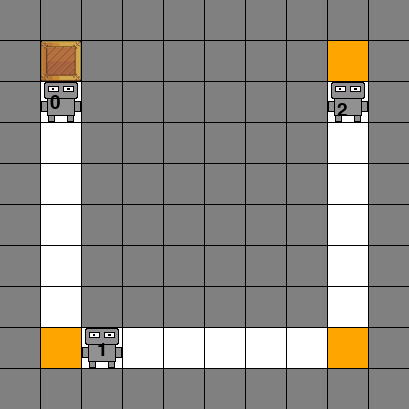
\includegraphics[width=0.154\textwidth]{figures/moving_company_1.png}
  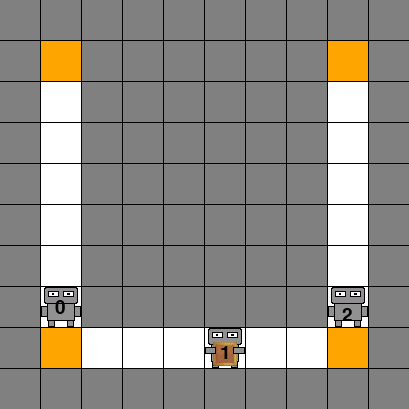
\includegraphics[width=0.154\textwidth]{figures/moving_company_2.png}
  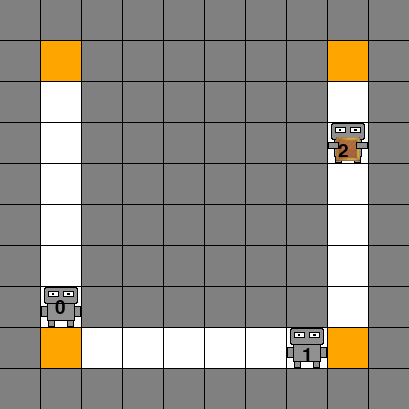
\includegraphics[width=0.154\textwidth]{figures/moving_company_3.png}
  \caption{Rendus visuels de \emph{Moving Company} avec trois agents déménageurs et un paquet.}
  \label{fig:env_moving_company}
\end{figure}

\subsection{Utilisation de \emph{PRAHOM Wrapper}}

Au travers de \emph{Moving Company}, nous montrons les fonctionalités de \emph{PRAHOM Wrapper}. Le code utilisé est résumé dans \autoref{lst:wrapper_mc}.

\paragraph{Mise en place et configuration}

Après avoir instantié l'environnement \emph{Moving Company} (ligne TODO), nous définissions quelques relations connues entre des sous-historiques et des spécifications organisationelles connues (ligne TODO). De même nous définissons des contraintes d'organisation (ligne TODO). Ensuite, \emph{PRAHOM Wrapper} enveloppe l'environnement avec les éventuelles relations et les contraintes pré-établies (ligne TODO). Les contraintes et relations peuvent être des mapping ou des fonctions dans la mesure où les deux associent respectivement un agent à ses contraintes et un historique à des spécifications organisationelles connues.

Le concepteur peut aussi modifier les valeurs par défaut relatives aux: mode de respect des contraintes (correction externe, apprentissage, modification des politiques), les méthodes utilisées pour l'analyse des historiques (clustering de séquence, analyse de fréquence, identification de sous-séquence\dots), les différentes spécifications organisationelles attendues, les figures et supports associées aux spécifications générées (dendogramme, ACP, plan d'objectifs\dots).

\paragraph{Entrainement contrainte des agents}

Le concepteur peut procéder classiquement à l'apprentissage avec l'environnement envelopé comme dans n'importe quel environnement PettingZoo. Sinon il peut utiliser l'algorithme \emph{Proximal Policy Optimization} (PPO) integré nativement via la bibliothèque \emph{Stable BaseLines3}. Nous utilisons cette fonctionalité (ligne TODO) avec les paramètrage existant \textquote{PPO\_default} : un nombre d'itérations indéfini, un temps d'apprentissage de 2h, le mode apprentissage centralisé et éxécution décentralisée, pas d'optimisation des hyper-paramètres, la sauvegarde de la meilleure politique et la restauration à partir du dernier checkpoint s'il existe.

\emph{PRAHOM Wrapper} permet alors d'obliger les agents à respecter la contrainte donnée (ligne TODO). Ici, si l'$agent_0$ observe qu'un paquet se trouve dans la case supérieure à la sienne, il doit prendre le paquet (action $5$).

\paragraph{Génération et évaluation des spécificiations organisationnelles }

Nous générons ensuite les spécifications organisationelles selon le paramètrage par défaut consistant à générer et analyser des historiques conjoints joués sur 5 épisodes avec la meilleure politique apprise (ligne TODO).
\emph{PRAHOM Wrapper} prend en priorité en compte les relations déjà connues (ligne TODO). Ici, si on voit qu'un des historique des agents contient l'action $3$ (se déplacer par la gauche) alors cela correspond au role \textquote{horizontal\_mover}.

Si un historique n'est pas déjà associé à une spécification organisationelle, \emph{PRAHOM Wrapper} cherche à généraliser des roles non pré-établis par mesure de similarité entre les historiques des agents. Cela est présentement fait de plusieurs façons complémentaires : par clustering de séquence auquel un dendogramme associé est sauvergardé en accompagnement ; par recherche des K-voisins les plus proches des historiques auquel une ACP des historiques est proposé en accompagnement ; par analyse statistique (fréquences, variances des couples observation-action) à laquelle des diagrammes circulaires et d'autres visulations diverses sont proposés.

De même des sous-objectifs peuvent être généralisés de plusieurs façons complémentaires : par analyse de la fréquence des observations finales communes des agents jouant un même role. Un digramme de transition des observations clés est généré en accompagnement ; par analyse des états seuils récurrents déclenchant une amélioration notable de l'évolution de la récompense auquel un digramme de transition des états seuils est généré en accompagnement.

A partir des rôles et sous-objectifs obtenus, \emph{PRAHOM Wrapper} propose une façon empirique d'inferrer d'autres spécifications organisationnelles comme les compatibilités entre roles, les permissions et obligations.

\begin{lstlisting}[language=Python, caption={Utilisation synthétique de \emph{PRAHOM Wrapper} pour \emph{Moving Company}}, label={lst:wrapper_mc}]
from custom_envs.movingcompany import moving_company_v0
from prahom_wrapper import PrahomWrapper
env = moving_company_v0.parallel_env(render_mode="human")
def hist_to_specs(hist): return {"role": "horizontal_mover"} if "3" in [
    act for obs, act in hist.items()] else None
agt_to_cons_specs = {"agent_0": {"[0 5 0 0 2 0 0 1 0]": 5}}
env = PrahomWrapper(env, hist_to_specs, agt_to_cons_specs, "CORRECT", [
                    "sequence_clustering"], ["role", "plan"], ["dendogram", "PCA"])
env.train("PPO_default")
raw_specs, agent_to_specs = env.generate_specs()
\end{lstlisting}

\section{Conclusion}

\emph{PRAHOM Wrapper} vise à donner des moyens de contraindre l'apprentissage des agents et à determiner automatiquement les spécifications organisationnelles sur la base d'historiques en étant ainsi agnostique de l'algorithme MARL choisi.
La version actuelle met en jeu de premières techniques statistiques simples et d'apprentissage non-supervisé pour l'analyse des historiques conjoints pour identifier des spécifications organisationnelles notamment des rôles.

Cependant, ces techniques peuvent présenter des limitations pour l'identification des liens entre les rôles joués par les agents au travers de leurs communications ou représentations menant à des spécifications incomplètes.
Les travaux récents sur l'apprentissage hierarchique pourraient être une source d'inspiration pour aider à caractériser les stratégies émergentes tout au long de l’apprentissage de façon plus générale et complète.
À terme, nous visons également à améliorer l'applicabilité de \emph{PRAHOM Wrapper} en enrichissant son interface et son intégration dans des contextes industriels et de recherche.


% \begin{thebibliography}{9}
% {\small
% \bibitem{bar} U. Nexpert, \emph{Le livre,} Son Editeur, 1929.

% \bibitem{foo} I. Troiseu-Pami, Un article intéressant, \emph{Journal de
%     Spirou}, Vol. 17, pp. 1-100, 1987
% }
% \end{thebibliography}

% \section*{Remerciements}

% Ce travail est financé par Thales Land Air Systems dans le cadre des travaux conjoints de la chair Cyb'Air et de l'AICA IWG.

\section*{References}
\small
\bibliographystyle{abbrv}
\bibliography{references}


\end{document}

%%% Local Variables: 
%%% mode: latex
%%% TeX-SMAter: "jfsmaLatex"
%%% ispell-local-dictionary: "francais"
%%% TeX-command-extra-options: "-shell-escape"
%%% End: 